\documentclass[tikz,border=2pt]{standalone}
\usepackage{amsmath}
\usepackage{pgfplots}
\pgfplotsset{compat=1.18}
\usepgfplotslibrary{fillbetween}
\usetikzlibrary{calc}

\begin{document}
% f(x)=x/2, F(x)=x^2/4, a=1, b=3. The integral and F(b)-F(a) both equal 2.
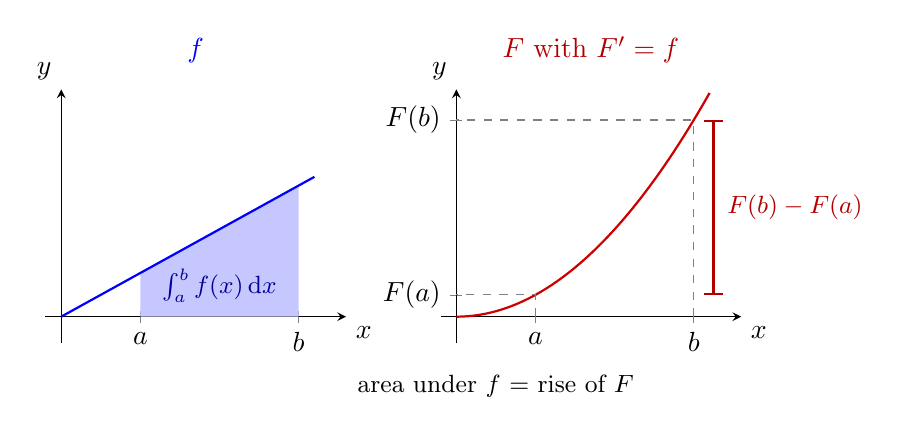
\begin{tikzpicture}
	\begin{axis}[
		name=left,
		axis lines=middle,
		xmin=-0.2, xmax=3.6,
		ymin=-0.3, ymax=2.6,
		xtick={1,3}, xticklabels={$a$,$b$},
		ytick=\empty,
		xlabel={$x$}, ylabel={$y$},
		xlabel style={below right}, ylabel style={above left},
		samples=120, smooth, clip=false,
		width=5.4cm, height=4.8cm,
		title={$f$}, title style={blue}
		]
		\addplot[name path=f, thick, blue, domain=0:3.2] {x/2};
		\addplot[name path=ax, draw=none, domain=0:3.2] {0};
		\addplot[blue!22] fill between[of=f and ax, soft clip={domain=1:3}];
		\node[blue!60!black, font=\small] at (axis cs:2.0,0.35) {$\int_a^b f(x)\,\mathrm{d}x$};
	\end{axis}
	\begin{axis}[
		at={(left.east)}, anchor=west, xshift=1.2cm,
		axis lines=middle,
		xmin=-0.2, xmax=3.6,
		ymin=-0.3, ymax=2.6,
		xtick={1,3}, xticklabels={$a$,$b$},
		ytick={0.25,2.25}, yticklabels={$F(a)$,$F(b)$},
		xlabel={$x$}, ylabel={$y$},
		xlabel style={below right}, ylabel style={above left},
		samples=120, smooth, clip=false,
		width=5.4cm, height=4.8cm,
		title={$F$ with $F'=f$}, title style={red!70!black}
		]
		\addplot[thick, red!80!black, domain=0:3.2] {x^2/4};
		\draw[dashed, gray] (axis cs:1,0) -- (axis cs:1,0.25) -- (axis cs:0,0.25);
		\draw[dashed, gray] (axis cs:3,0) -- (axis cs:3,2.25) -- (axis cs:0,2.25);
		\draw[red!70!black, thick, |-|] (axis cs:3.25,0.25) -- (axis cs:3.25,2.25);
		\node[red!70!black, anchor=west, font=\small] at (axis cs:3.3,1.25) {$F(b)-F(a)$};
	\end{axis}
	\node[font=\small] at ($(left.south east)+(1.9,-0.55)$) {area under $f$ $=$ rise of $F$};
\end{tikzpicture}
\end{document}
